\documentclass{article}
%\documentclass{standalone}
%\documentclass[conference]{IEEEtran}
\usepackage[a2paper]{geometry}

\usepackage{subcaption}
\usepackage{graphicx}
\usepackage{cite}
\usepackage{amsmath,amssymb,amsfonts}
%\usepackage{algorithmic}
\usepackage{enumitem}
\usepackage{lipsum}
\usepackage[draft]{hyperref}
\usepackage{pgfplotstable}
\usepackage[T1]{fontenc}% http://ctan.org/pkg/fontenc
\usepackage{subcaption}
%\usepackage{subfig}% http://ctan.org/pkg/subfig
\usepackage{siunitx}
\usepackage{gensymb}
\usepackage{float}
\floatstyle{plaintop}
\restylefloat{table}
\newlength\mylen
\settowidth\mylen{\textbf{Case~5.}}
\newlist{mycases}{enumerate}{1}
\setlist[mycases,1]{label=\textbf{Case~\arabic*.}, 
	labelwidth=\dimexpr-\mylen-\labelsep\relax,leftmargin=0pt,align=right}
\usepackage{enumitem}
\usepackage{eurosym}
\usepackage{amstext} % for \text
\usepackage{longtable}
\usepackage{multirow}
\usepackage{arydshln}
\usepackage{tabularx}
\usepackage{tikz}
\usepackage{pgfplots}
\usepackage{tikz}
\usetikzlibrary{arrows,shapes, calc, fit, positioning}
\usepackage{pgfplots}
\usepackage{dblfloatfix}
\usepackage{cleveref}
\usepackage{placeins}
\usepackage{booktabs}

\usepackage{graphicx}
\graphicspath{{./gfx/}}
\DeclareGraphicsExtensions{.pdf,.jpeg,.png}

\DeclareRobustCommand{\officialeuro}{%
	\ifmmode\expandafter\text\fi
	{\fontencoding{U}\fontfamily{eurosym}\selectfont e}}

\usepackage{fontenc}
\usepackage{siunitx}
\usepackage{booktabs}
\usepackage{colortbl}
\usepackage[numbers]{natbib}


\newcommand\SEB[1]{\textsubscript{#1}}
\def\RC{\rowcolor{gray!10}}
\renewcommand{\arraystretch}{1.2}

%\setlength{\intextsep}{10pt plus 2pt minus 2pt}

%\usepackage{textcomp}
%\usepackage[keeplastbox]{flushend} 

%\usepackage{multirow}
%\usepackage{acro}
%\def\BibTeX{{\rm B\kern-.05em{\sc i\kern-.025em b}\kern-.08em
%    T\kern-.1667em\lower.7ex\hbox{E}\kern-.125emX}}
%
%
%\usepackage[numbers,sort&compress]{natbib}
%\newcommand{\alignedintertext}[1]{%
%	\noalign{%
%		\vskip\belowdisplayshortskip
%		\vtop{\hsize=\linewidth#1\par
%			\expandafter}%
%		\expandafter\prevdepth\the\prevdepth
%	}%
%}
\usepackage{float}
\usepackage{algorithm}
\usepackage[noend]{algpseudocode}
\usepackage{tikz}
\usetikzlibrary{trees}
\newenvironment{subgroup}
{$\left\{\tabular{l}}
{\endtabular\right.$}
\usepackage{hyphenat}

\title{%\vspace{-1.5cm}            % Another way to do
	\Huge {Key features responsible for the proper diagnosis of PTSD}}

\author{\Large Ishan Khatri}
\begin{document}\sloppy
\maketitle
%\section{title}
%this is to be done
\centering

\begin{table}[H]

\begin{tabular}{|p{4cm}|p{4cm}|}
	\centering
\textbf{\Large Each Individual patient}
\end{tabular}
\begin{subgroup}
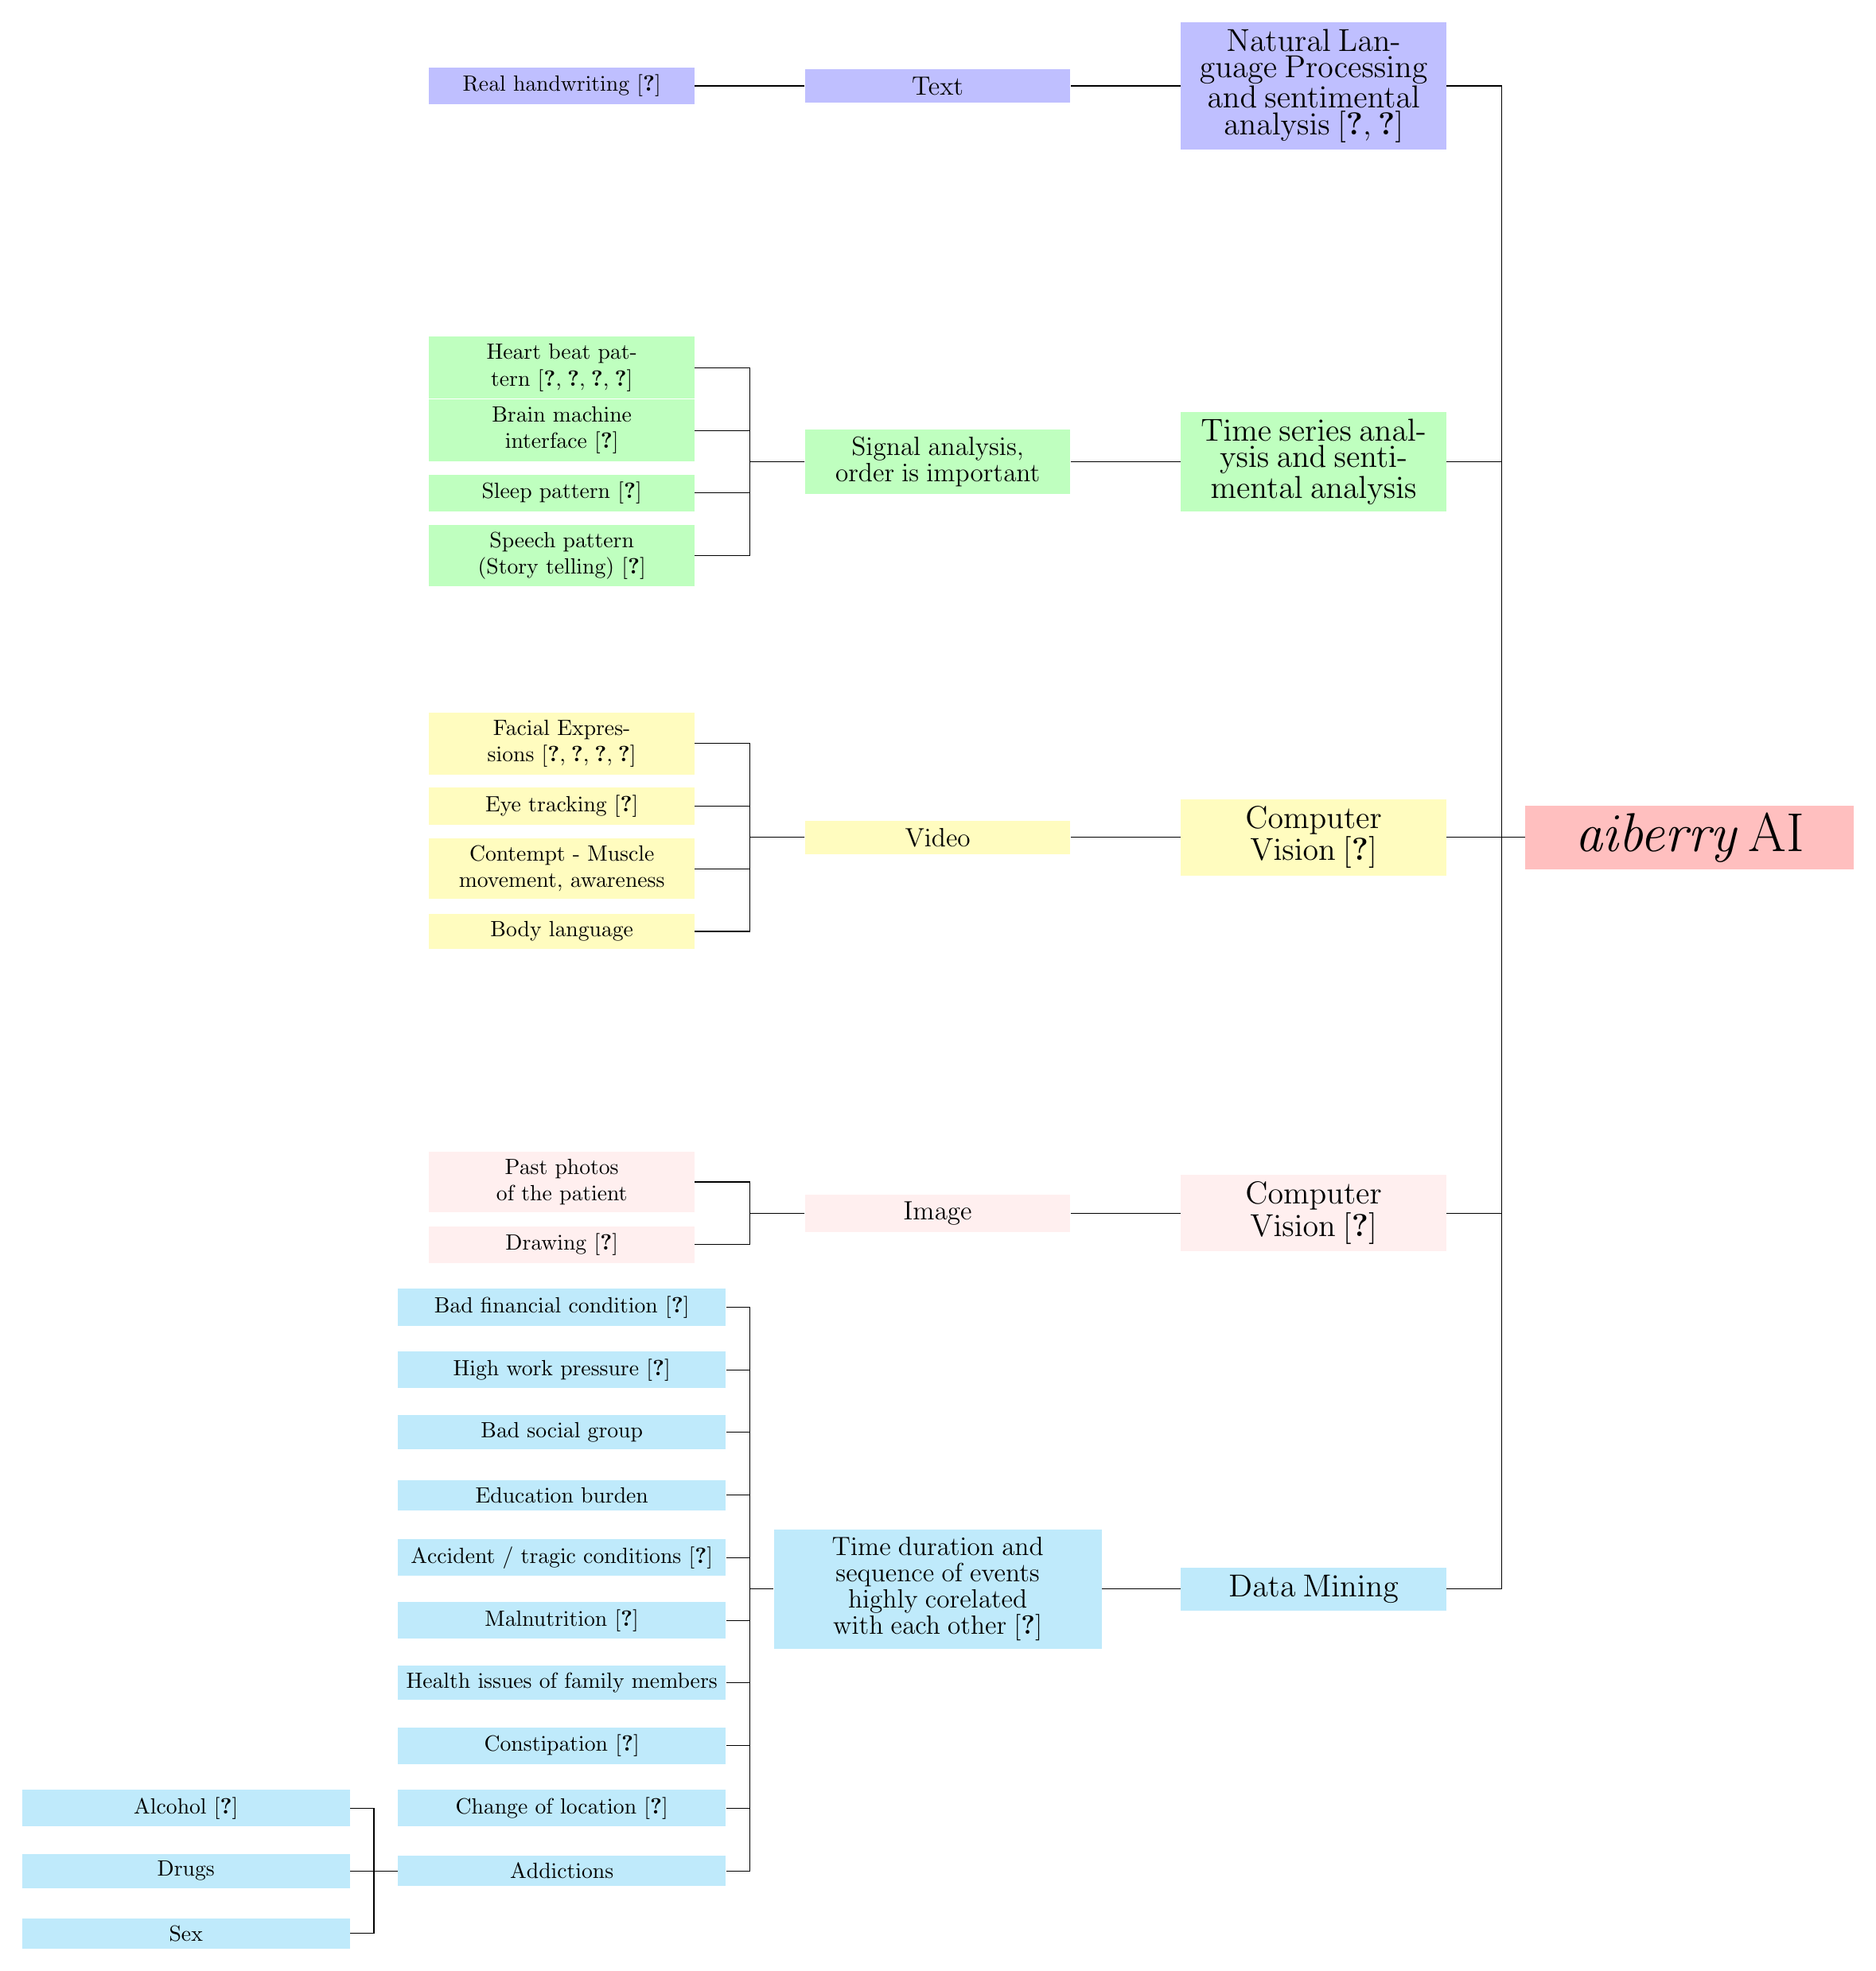
\begin{tikzpicture}[edge from parent fork left,grow=left,level distance=6cm,level 1/.style={sibling distance=6cm},
level 2/.style={sibling distance=1cm}, level 3/.style={sibling distance=1cm}]
\node[align=center, fill=red!25, text width=5cm] {\Huge \textit{aiberry} AI}
child {node [align=center, fill=blue!25,text width=4cm]{\Large Natural Language Processing and sentimental analysis \cite{nlphoward2013approach,bourla2018ptsd}}
	child {node [align=center, fill=blue!25,text width=4cm]{\large Text}
			child {node [align=center, fill=blue!25,text width=4cm]{Real handwriting \cite{handwriting2015}}}}}
%			child {node [align=center, fill=blue!25,text width=4cm]{Digital}}}}
child {node [align=center, fill=green!25,text width=4cm]{\Large Time series analysis and sentimental analysis}
	child {node [align=center, fill=green!25,text width=4cm]{\large Signal analysis, order is important}
		child {node [align=center, fill=green!25,text width=4cm]{Heart beat pattern \cite{heart2016,heartsmokealcohol2014,heart2010riganello, heartkibler2009hypertension}}}
		child {node [align=center, fill=green!25,text width=4cm]{Brain machine interface \cite{brainsignals2019butt}}}
		child {node [align=center, fill=green!25,text width=4cm]{Sleep pattern \cite{heartsmokealcohol2014}}}
		child {node [align=center, fill=green!25,text width=4cm]{Speech pattern (Story telling) \cite{speechvan2010telling}}}}}
child {node [align=center, fill=yellow!25,text width=4cm]{\Large Computer Vision \cite{cosic2013computer}}
	child {node [align=center, fill=yellow!25,text width=4cm]{\large Video}
		child {node [align=center, fill=yellow!25,text width=4cm]{Facial Expressions \cite{facearmony2005amygdala,facegarrett2012brain,facefujiwara2015association, faceshin2006amygdala}}}
		child {node [align=center, fill=yellow!25,text width=4cm]{Eye tracking \cite{eyepowers2019attention}}}
		child {node [align=center, fill=yellow!25,text width=4cm][text width=4cm]{Contempt - Muscle movement, awareness}}
		child {node [align=center, fill=yellow!25,text width=4cm]{Body language}}}}
child {node [align=center, fill=pink!25,text width=4cm]{\Large Computer Vision \cite{cosic2013computer}}
	child {node [align=center, fill=pink!25,text width=4cm]{\large Image}
		child {node [align=center, fill=pink!25,text width=4cm]{Past photos of the patient}}
		child {node [align=center, fill=pink!25,text width=4cm]{Drawing \cite{drawingspring2004thirty}}}}}
child {node [align=center, fill=cyan!25,text width=4cm]{\Large Data Mining}
	child {node [align=center, fill=cyan!25,text width=5cm]{\large Time duration and sequence of events highly corelated with each other \cite{kessler1995posttraumatic}}
		child {node [align=center, fill=cyan!25,text width=5cm]{Bad financial condition \cite{financialptsd2005}}}
		child {node [align=center, fill=cyan!25,text width=5cm]{High work pressure \cite{workchan2004influence}}}
		child {node [align=center, fill=cyan!25,text width=5cm]{Bad social group}}
		child {node [align=center, fill=cyan!25,text width=5cm]{Education burden}}
		child {node [align=center, fill=cyan!25,text width=5cm]{Accident / tragic conditions \cite{joyce2007language}}}
		child {node [align=center, fill=cyan!25,text width=5cm]{Malnutrition \cite{malnutritionde2012impact}}}
		child {node [align=center, fill=cyan!25,text width=5cm]{Health issues of family members}}
		child {node [align=center, fill=cyan!25,text width=5cm]{Constipation \cite{ibsptsd2019}}}
		child {node [align=center, fill=cyan!25,text width=5cm]{Change of location \cite{joyce2007language}}}
		child {node [align=center, fill=cyan!25,text width=5cm]{Addictions}
			child {node [align=center, fill=cyan!25,text width=5cm]{Alcohol \cite{heartsmokealcohol2014}}}
			child {node [align=center, fill=cyan!25,text width=5cm]{Drugs}}
			child {node [align=center, fill=cyan!25,text width=5cm]{Sex}}}}};
\end{tikzpicture}
\end{subgroup}
\end{table}
%\bibliographystyle{srt}
%\documentclass{article}
%\documentclass{standalone}
%\documentclass[conference]{IEEEtran}
\usepackage[a2paper]{geometry}

\usepackage{subcaption}
\usepackage{graphicx}
\usepackage{cite}
\usepackage{amsmath,amssymb,amsfonts}
%\usepackage{algorithmic}
\usepackage{enumitem}
\usepackage{lipsum}
\usepackage[draft]{hyperref}
\usepackage{pgfplotstable}
\usepackage[T1]{fontenc}% http://ctan.org/pkg/fontenc
\usepackage{subcaption}
%\usepackage{subfig}% http://ctan.org/pkg/subfig
\usepackage{siunitx}
\usepackage{gensymb}
\usepackage{float}
\floatstyle{plaintop}
\restylefloat{table}
\newlength\mylen
\settowidth\mylen{\textbf{Case~5.}}
\newlist{mycases}{enumerate}{1}
\setlist[mycases,1]{label=\textbf{Case~\arabic*.}, 
	labelwidth=\dimexpr-\mylen-\labelsep\relax,leftmargin=0pt,align=right}
\usepackage{enumitem}
\usepackage{eurosym}
\usepackage{amstext} % for \text
\usepackage{longtable}
\usepackage{multirow}
\usepackage{arydshln}
\usepackage{tabularx}
\usepackage{tikz}
\usepackage{pgfplots}
\usepackage{tikz}
\usetikzlibrary{arrows,shapes, calc, fit, positioning}
\usepackage{pgfplots}
\usepackage{dblfloatfix}
\usepackage{cleveref}
\usepackage{placeins}
\usepackage{booktabs}

\usepackage{graphicx}
\graphicspath{{./gfx/}}
\DeclareGraphicsExtensions{.pdf,.jpeg,.png}

\DeclareRobustCommand{\officialeuro}{%
	\ifmmode\expandafter\text\fi
	{\fontencoding{U}\fontfamily{eurosym}\selectfont e}}

\usepackage{fontenc}
\usepackage{siunitx}
\usepackage{booktabs}
\usepackage{colortbl}
\usepackage[numbers]{natbib}


\newcommand\SEB[1]{\textsubscript{#1}}
\def\RC{\rowcolor{gray!10}}
\renewcommand{\arraystretch}{1.2}

%\setlength{\intextsep}{10pt plus 2pt minus 2pt}

%\usepackage{textcomp}
%\usepackage[keeplastbox]{flushend} 

%\usepackage{multirow}
%\usepackage{acro}
%\def\BibTeX{{\rm B\kern-.05em{\sc i\kern-.025em b}\kern-.08em
%    T\kern-.1667em\lower.7ex\hbox{E}\kern-.125emX}}
%
%
%\usepackage[numbers,sort&compress]{natbib}
%\newcommand{\alignedintertext}[1]{%
%	\noalign{%
%		\vskip\belowdisplayshortskip
%		\vtop{\hsize=\linewidth#1\par
%			\expandafter}%
%		\expandafter\prevdepth\the\prevdepth
%	}%
%}
\usepackage{float}
\usepackage{algorithm}
\usepackage[noend]{algpseudocode}
\usepackage{tikz}
\usetikzlibrary{trees}
\newenvironment{subgroup}
{$\left\{\tabular{l}}
{\endtabular\right.$}
\usepackage{hyphenat}

\title{%\vspace{-1.5cm}            % Another way to do
	\Huge {Key features responsible for the proper diagnosis of PTSD}}

\author{\Large Ishan Khatri}
\begin{document}\sloppy
\maketitle
%\section{title}
%this is to be done
\centering

\begin{table}[H]

\begin{tabular}{|p{4cm}|p{4cm}|}
	\centering
\textbf{\Large Each Individual patient}
\end{tabular}
\begin{subgroup}
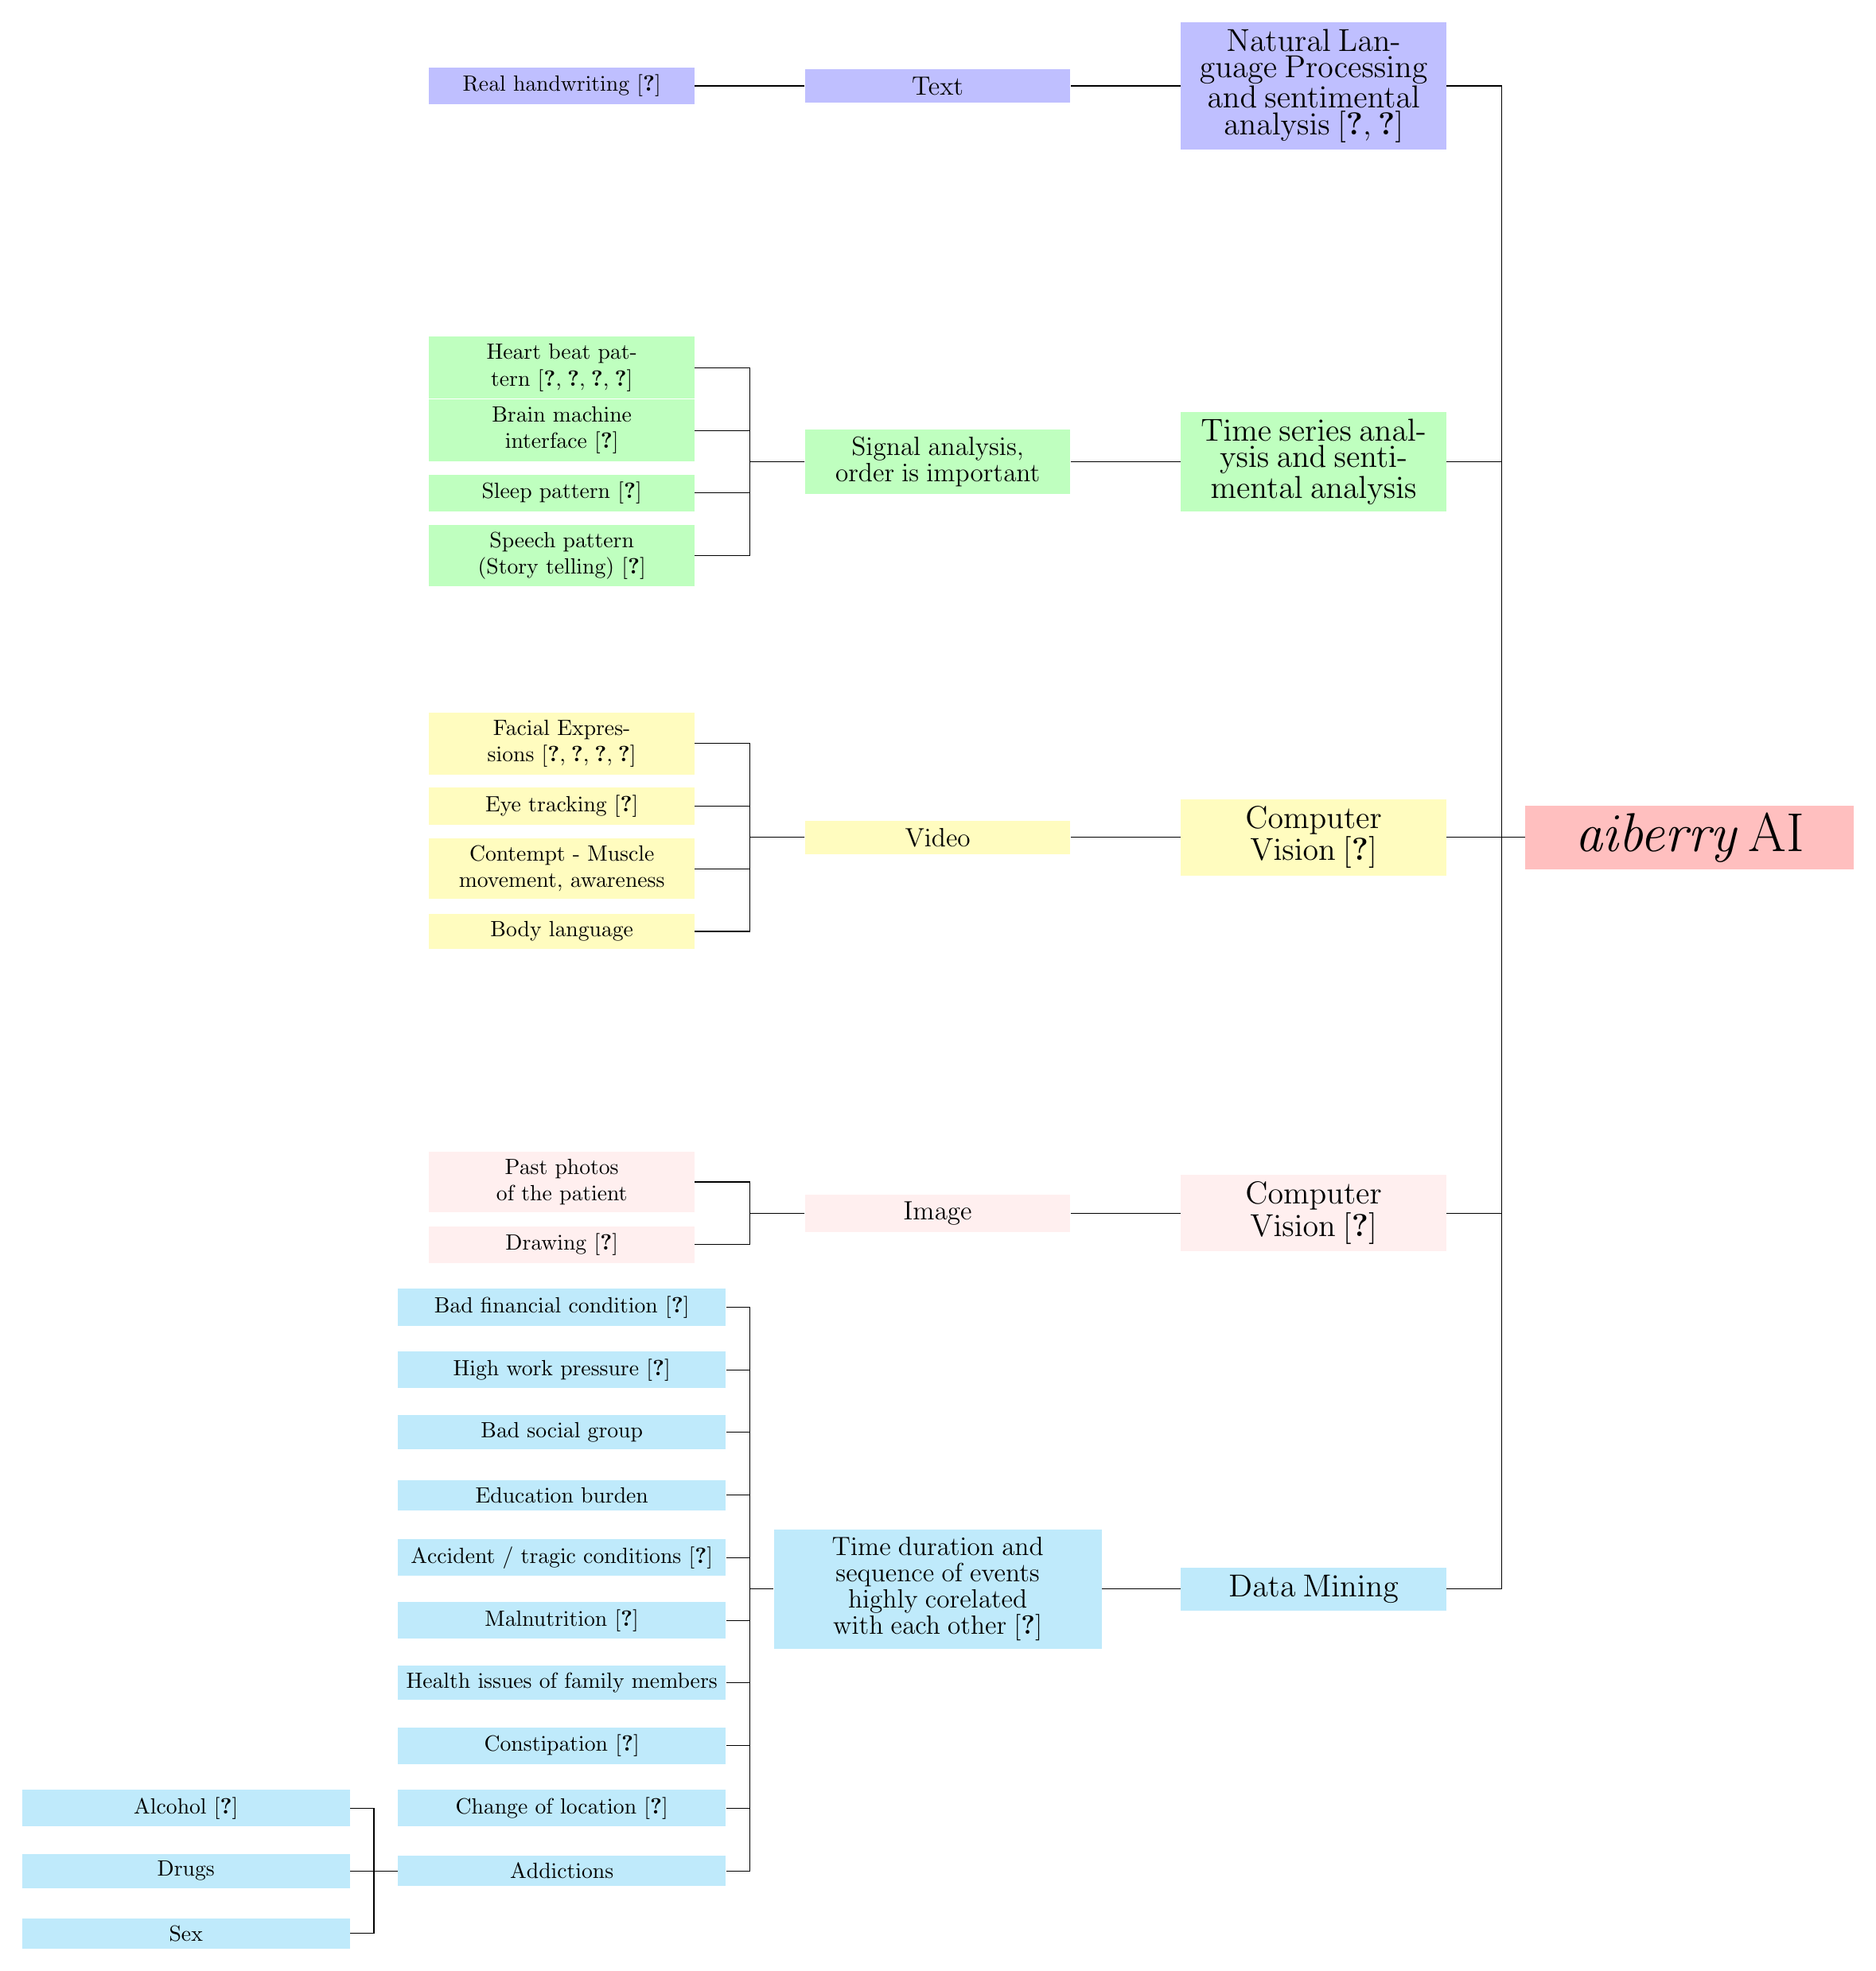
\begin{tikzpicture}[edge from parent fork left,grow=left,level distance=6cm,level 1/.style={sibling distance=6cm},
level 2/.style={sibling distance=1cm}, level 3/.style={sibling distance=1cm}]
\node[align=center, fill=red!25, text width=5cm] {\Huge \textit{aiberry} AI}
child {node [align=center, fill=blue!25,text width=4cm]{\Large Natural Language Processing and sentimental analysis \cite{nlphoward2013approach,bourla2018ptsd}}
	child {node [align=center, fill=blue!25,text width=4cm]{\large Text}
			child {node [align=center, fill=blue!25,text width=4cm]{Real handwriting \cite{handwriting2015}}}}}
%			child {node [align=center, fill=blue!25,text width=4cm]{Digital}}}}
child {node [align=center, fill=green!25,text width=4cm]{\Large Time series analysis and sentimental analysis}
	child {node [align=center, fill=green!25,text width=4cm]{\large Signal analysis, order is important}
		child {node [align=center, fill=green!25,text width=4cm]{Heart beat pattern \cite{heart2016,heartsmokealcohol2014,heart2010riganello, heartkibler2009hypertension}}}
		child {node [align=center, fill=green!25,text width=4cm]{Brain machine interface \cite{brainsignals2019butt}}}
		child {node [align=center, fill=green!25,text width=4cm]{Sleep pattern \cite{heartsmokealcohol2014}}}
		child {node [align=center, fill=green!25,text width=4cm]{Speech pattern (Story telling) \cite{speechvan2010telling}}}}}
child {node [align=center, fill=yellow!25,text width=4cm]{\Large Computer Vision \cite{cosic2013computer}}
	child {node [align=center, fill=yellow!25,text width=4cm]{\large Video}
		child {node [align=center, fill=yellow!25,text width=4cm]{Facial Expressions \cite{facearmony2005amygdala,facegarrett2012brain,facefujiwara2015association, faceshin2006amygdala}}}
		child {node [align=center, fill=yellow!25,text width=4cm]{Eye tracking \cite{eyepowers2019attention}}}
		child {node [align=center, fill=yellow!25,text width=4cm][text width=4cm]{Contempt - Muscle movement, awareness}}
		child {node [align=center, fill=yellow!25,text width=4cm]{Body language}}}}
child {node [align=center, fill=pink!25,text width=4cm]{\Large Computer Vision \cite{cosic2013computer}}
	child {node [align=center, fill=pink!25,text width=4cm]{\large Image}
		child {node [align=center, fill=pink!25,text width=4cm]{Past photos of the patient}}
		child {node [align=center, fill=pink!25,text width=4cm]{Drawing \cite{drawingspring2004thirty}}}}}
child {node [align=center, fill=cyan!25,text width=4cm]{\Large Data Mining}
	child {node [align=center, fill=cyan!25,text width=5cm]{\large Time duration and sequence of events highly corelated with each other \cite{kessler1995posttraumatic}}
		child {node [align=center, fill=cyan!25,text width=5cm]{Bad financial condition \cite{financialptsd2005}}}
		child {node [align=center, fill=cyan!25,text width=5cm]{High work pressure \cite{workchan2004influence}}}
		child {node [align=center, fill=cyan!25,text width=5cm]{Bad social group}}
		child {node [align=center, fill=cyan!25,text width=5cm]{Education burden}}
		child {node [align=center, fill=cyan!25,text width=5cm]{Accident / tragic conditions \cite{joyce2007language}}}
		child {node [align=center, fill=cyan!25,text width=5cm]{Malnutrition \cite{malnutritionde2012impact}}}
		child {node [align=center, fill=cyan!25,text width=5cm]{Health issues of family members}}
		child {node [align=center, fill=cyan!25,text width=5cm]{Constipation \cite{ibsptsd2019}}}
		child {node [align=center, fill=cyan!25,text width=5cm]{Change of location \cite{joyce2007language}}}
		child {node [align=center, fill=cyan!25,text width=5cm]{Addictions}
			child {node [align=center, fill=cyan!25,text width=5cm]{Alcohol \cite{heartsmokealcohol2014}}}
			child {node [align=center, fill=cyan!25,text width=5cm]{Drugs}}
			child {node [align=center, fill=cyan!25,text width=5cm]{Sex}}}}};
\end{tikzpicture}
\end{subgroup}
\end{table}
%\bibliographystyle{srt}
%\documentclass{article}
%\documentclass{standalone}
%\documentclass[conference]{IEEEtran}
\usepackage[a2paper]{geometry}

\usepackage{subcaption}
\usepackage{graphicx}
\usepackage{cite}
\usepackage{amsmath,amssymb,amsfonts}
%\usepackage{algorithmic}
\usepackage{enumitem}
\usepackage{lipsum}
\usepackage[draft]{hyperref}
\usepackage{pgfplotstable}
\usepackage[T1]{fontenc}% http://ctan.org/pkg/fontenc
\usepackage{subcaption}
%\usepackage{subfig}% http://ctan.org/pkg/subfig
\usepackage{siunitx}
\usepackage{gensymb}
\usepackage{float}
\floatstyle{plaintop}
\restylefloat{table}
\newlength\mylen
\settowidth\mylen{\textbf{Case~5.}}
\newlist{mycases}{enumerate}{1}
\setlist[mycases,1]{label=\textbf{Case~\arabic*.}, 
	labelwidth=\dimexpr-\mylen-\labelsep\relax,leftmargin=0pt,align=right}
\usepackage{enumitem}
\usepackage{eurosym}
\usepackage{amstext} % for \text
\usepackage{longtable}
\usepackage{multirow}
\usepackage{arydshln}
\usepackage{tabularx}
\usepackage{tikz}
\usepackage{pgfplots}
\usepackage{tikz}
\usetikzlibrary{arrows,shapes, calc, fit, positioning}
\usepackage{pgfplots}
\usepackage{dblfloatfix}
\usepackage{cleveref}
\usepackage{placeins}
\usepackage{booktabs}

\usepackage{graphicx}
\graphicspath{{./gfx/}}
\DeclareGraphicsExtensions{.pdf,.jpeg,.png}

\DeclareRobustCommand{\officialeuro}{%
	\ifmmode\expandafter\text\fi
	{\fontencoding{U}\fontfamily{eurosym}\selectfont e}}

\usepackage{fontenc}
\usepackage{siunitx}
\usepackage{booktabs}
\usepackage{colortbl}
\usepackage[numbers]{natbib}


\newcommand\SEB[1]{\textsubscript{#1}}
\def\RC{\rowcolor{gray!10}}
\renewcommand{\arraystretch}{1.2}

%\setlength{\intextsep}{10pt plus 2pt minus 2pt}

%\usepackage{textcomp}
%\usepackage[keeplastbox]{flushend} 

%\usepackage{multirow}
%\usepackage{acro}
%\def\BibTeX{{\rm B\kern-.05em{\sc i\kern-.025em b}\kern-.08em
%    T\kern-.1667em\lower.7ex\hbox{E}\kern-.125emX}}
%
%
%\usepackage[numbers,sort&compress]{natbib}
%\newcommand{\alignedintertext}[1]{%
%	\noalign{%
%		\vskip\belowdisplayshortskip
%		\vtop{\hsize=\linewidth#1\par
%			\expandafter}%
%		\expandafter\prevdepth\the\prevdepth
%	}%
%}
\usepackage{float}
\usepackage{algorithm}
\usepackage[noend]{algpseudocode}
\usepackage{tikz}
\usetikzlibrary{trees}
\newenvironment{subgroup}
{$\left\{\tabular{l}}
{\endtabular\right.$}
\usepackage{hyphenat}

\title{%\vspace{-1.5cm}            % Another way to do
	\Huge {Key features responsible for the proper diagnosis of PTSD}}

\author{\Large Ishan Khatri}
\begin{document}\sloppy
\maketitle
%\section{title}
%this is to be done
\centering

\begin{table}[H]

\begin{tabular}{|p{4cm}|p{4cm}|}
	\centering
\textbf{\Large Each Individual patient}
\end{tabular}
\begin{subgroup}
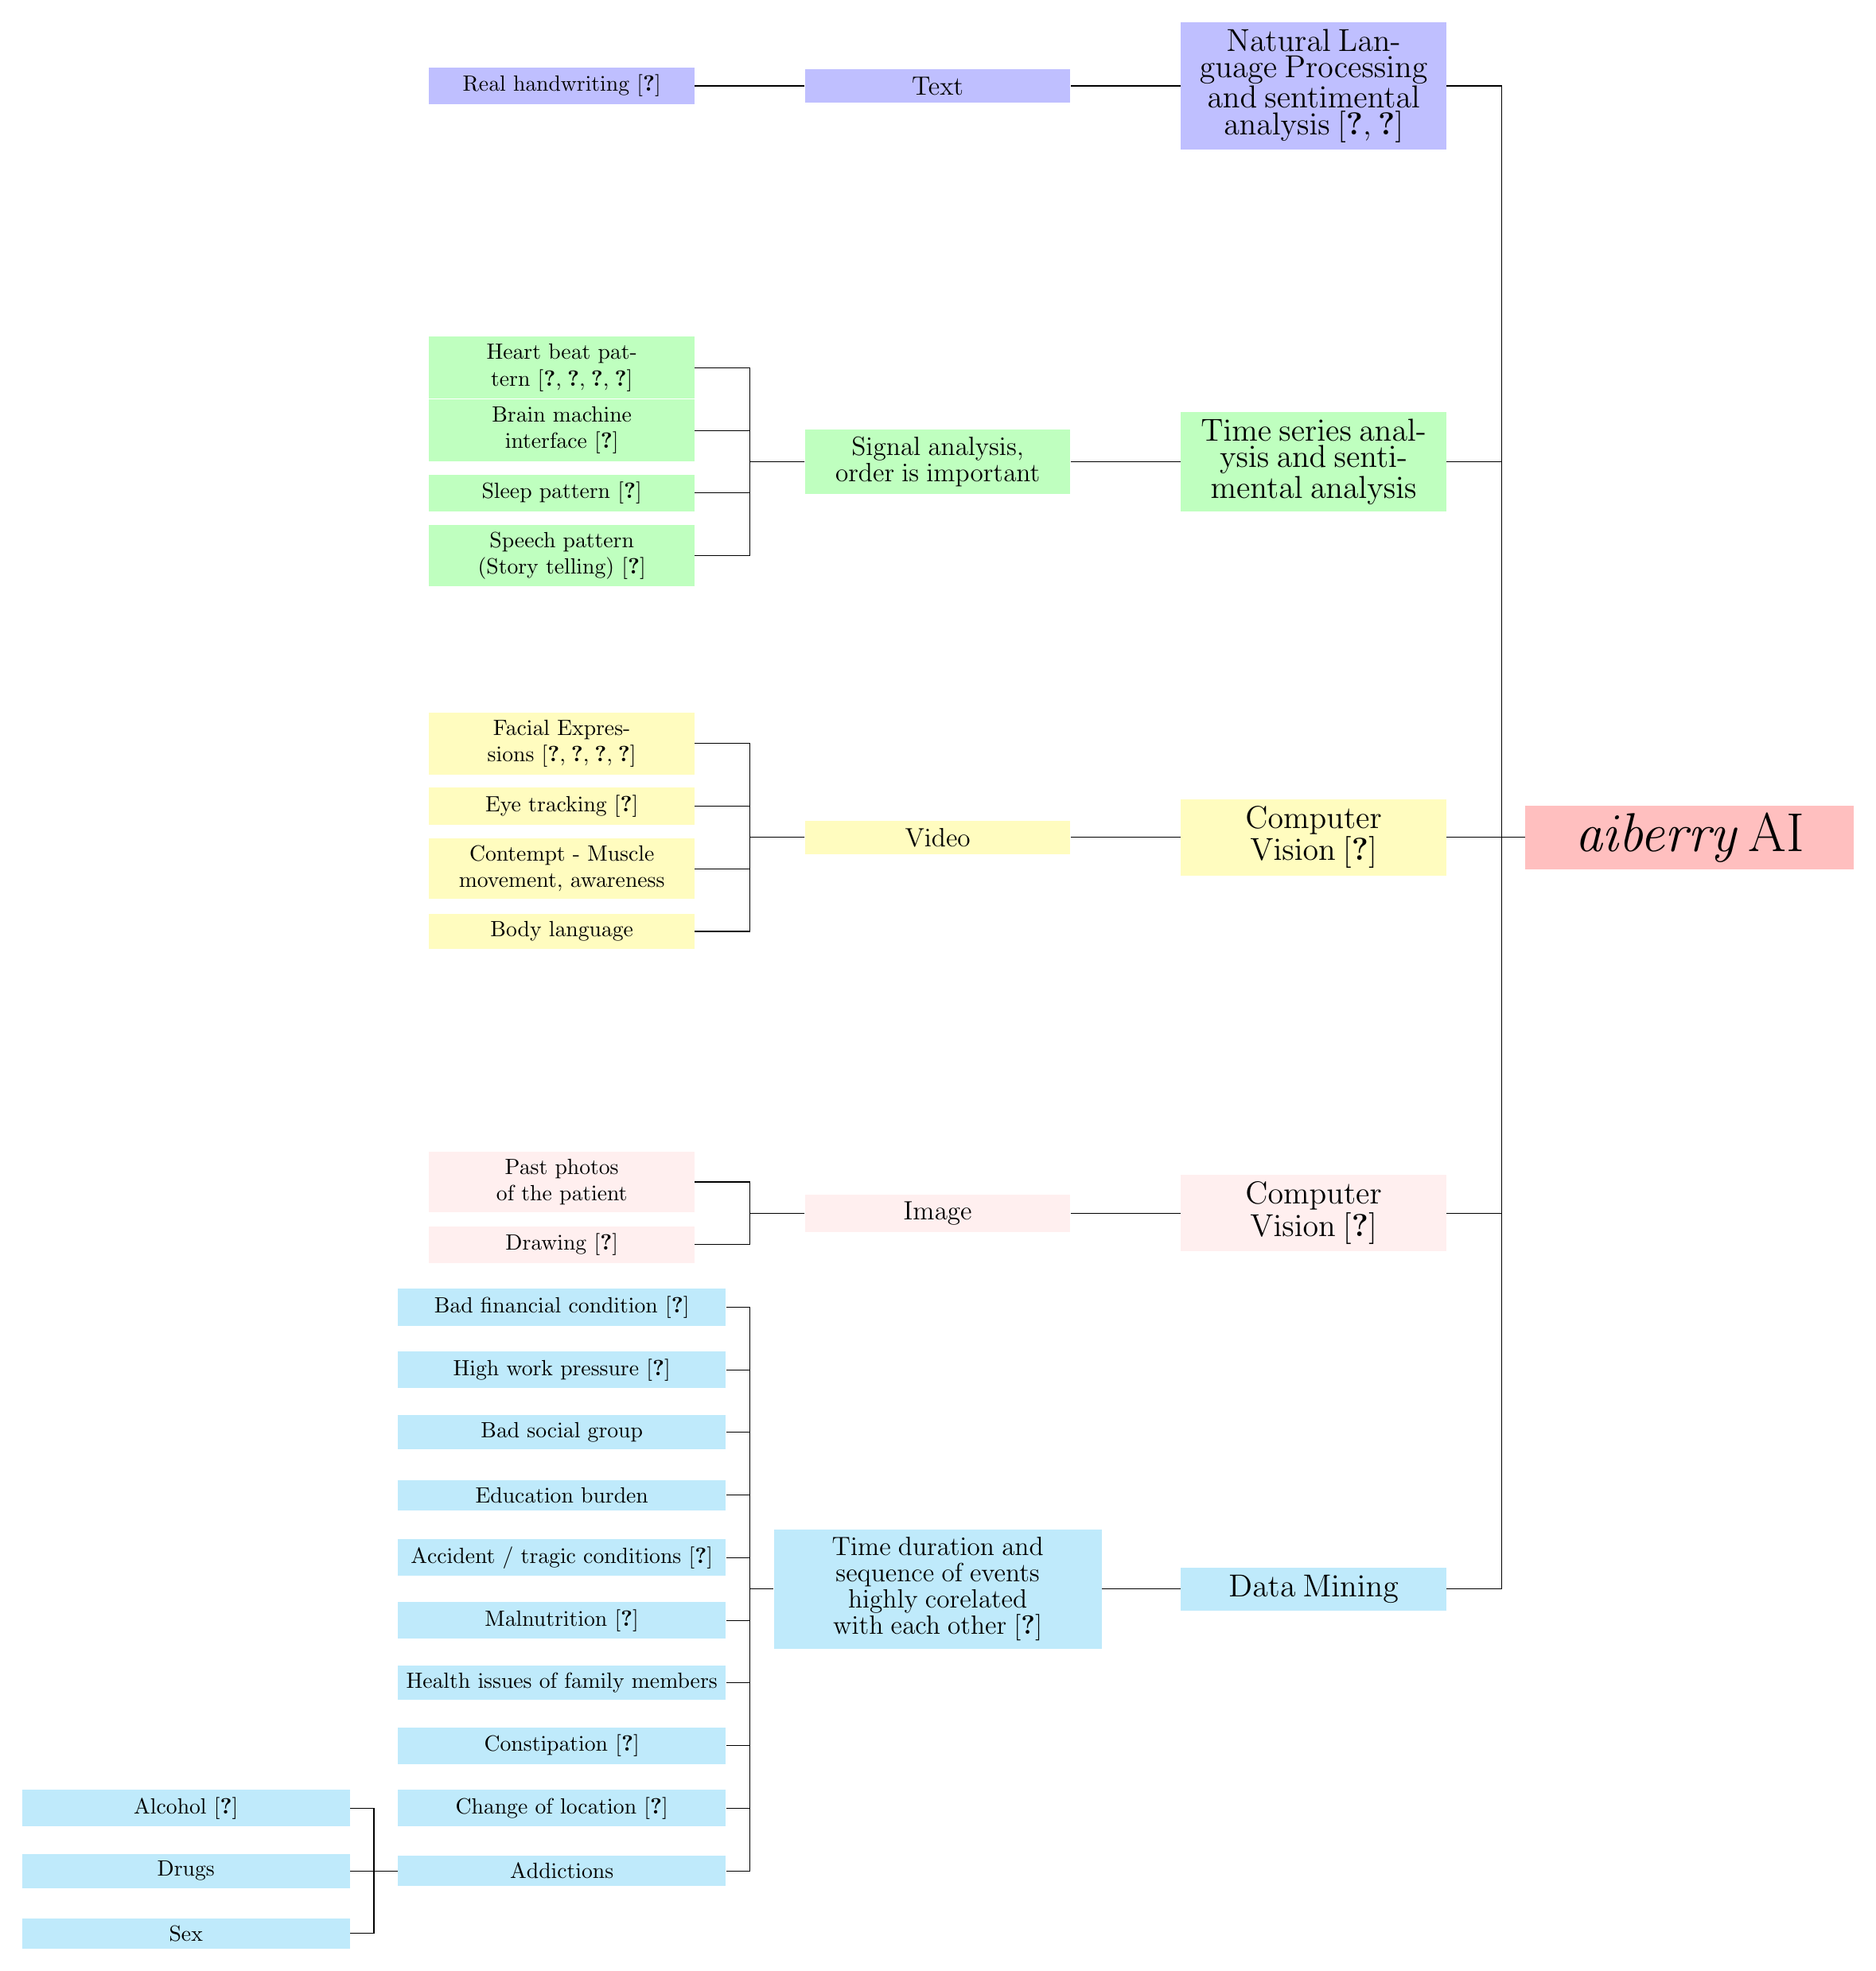
\begin{tikzpicture}[edge from parent fork left,grow=left,level distance=6cm,level 1/.style={sibling distance=6cm},
level 2/.style={sibling distance=1cm}, level 3/.style={sibling distance=1cm}]
\node[align=center, fill=red!25, text width=5cm] {\Huge \textit{aiberry} AI}
child {node [align=center, fill=blue!25,text width=4cm]{\Large Natural Language Processing and sentimental analysis \cite{nlphoward2013approach,bourla2018ptsd}}
	child {node [align=center, fill=blue!25,text width=4cm]{\large Text}
			child {node [align=center, fill=blue!25,text width=4cm]{Real handwriting \cite{handwriting2015}}}}}
%			child {node [align=center, fill=blue!25,text width=4cm]{Digital}}}}
child {node [align=center, fill=green!25,text width=4cm]{\Large Time series analysis and sentimental analysis}
	child {node [align=center, fill=green!25,text width=4cm]{\large Signal analysis, order is important}
		child {node [align=center, fill=green!25,text width=4cm]{Heart beat pattern \cite{heart2016,heartsmokealcohol2014,heart2010riganello, heartkibler2009hypertension}}}
		child {node [align=center, fill=green!25,text width=4cm]{Brain machine interface \cite{brainsignals2019butt}}}
		child {node [align=center, fill=green!25,text width=4cm]{Sleep pattern \cite{heartsmokealcohol2014}}}
		child {node [align=center, fill=green!25,text width=4cm]{Speech pattern (Story telling) \cite{speechvan2010telling}}}}}
child {node [align=center, fill=yellow!25,text width=4cm]{\Large Computer Vision \cite{cosic2013computer}}
	child {node [align=center, fill=yellow!25,text width=4cm]{\large Video}
		child {node [align=center, fill=yellow!25,text width=4cm]{Facial Expressions \cite{facearmony2005amygdala,facegarrett2012brain,facefujiwara2015association, faceshin2006amygdala}}}
		child {node [align=center, fill=yellow!25,text width=4cm]{Eye tracking \cite{eyepowers2019attention}}}
		child {node [align=center, fill=yellow!25,text width=4cm][text width=4cm]{Contempt - Muscle movement, awareness}}
		child {node [align=center, fill=yellow!25,text width=4cm]{Body language}}}}
child {node [align=center, fill=pink!25,text width=4cm]{\Large Computer Vision \cite{cosic2013computer}}
	child {node [align=center, fill=pink!25,text width=4cm]{\large Image}
		child {node [align=center, fill=pink!25,text width=4cm]{Past photos of the patient}}
		child {node [align=center, fill=pink!25,text width=4cm]{Drawing \cite{drawingspring2004thirty}}}}}
child {node [align=center, fill=cyan!25,text width=4cm]{\Large Data Mining}
	child {node [align=center, fill=cyan!25,text width=5cm]{\large Time duration and sequence of events highly corelated with each other \cite{kessler1995posttraumatic}}
		child {node [align=center, fill=cyan!25,text width=5cm]{Bad financial condition \cite{financialptsd2005}}}
		child {node [align=center, fill=cyan!25,text width=5cm]{High work pressure \cite{workchan2004influence}}}
		child {node [align=center, fill=cyan!25,text width=5cm]{Bad social group}}
		child {node [align=center, fill=cyan!25,text width=5cm]{Education burden}}
		child {node [align=center, fill=cyan!25,text width=5cm]{Accident / tragic conditions \cite{joyce2007language}}}
		child {node [align=center, fill=cyan!25,text width=5cm]{Malnutrition \cite{malnutritionde2012impact}}}
		child {node [align=center, fill=cyan!25,text width=5cm]{Health issues of family members}}
		child {node [align=center, fill=cyan!25,text width=5cm]{Constipation \cite{ibsptsd2019}}}
		child {node [align=center, fill=cyan!25,text width=5cm]{Change of location \cite{joyce2007language}}}
		child {node [align=center, fill=cyan!25,text width=5cm]{Addictions}
			child {node [align=center, fill=cyan!25,text width=5cm]{Alcohol \cite{heartsmokealcohol2014}}}
			child {node [align=center, fill=cyan!25,text width=5cm]{Drugs}}
			child {node [align=center, fill=cyan!25,text width=5cm]{Sex}}}}};
\end{tikzpicture}
\end{subgroup}
\end{table}
%\bibliographystyle{srt}
%\documentclass{article}
%\documentclass{standalone}
%\documentclass[conference]{IEEEtran}
\usepackage[a2paper]{geometry}

\usepackage{subcaption}
\usepackage{graphicx}
\usepackage{cite}
\usepackage{amsmath,amssymb,amsfonts}
%\usepackage{algorithmic}
\usepackage{enumitem}
\usepackage{lipsum}
\usepackage[draft]{hyperref}
\usepackage{pgfplotstable}
\usepackage[T1]{fontenc}% http://ctan.org/pkg/fontenc
\usepackage{subcaption}
%\usepackage{subfig}% http://ctan.org/pkg/subfig
\usepackage{siunitx}
\usepackage{gensymb}
\usepackage{float}
\floatstyle{plaintop}
\restylefloat{table}
\newlength\mylen
\settowidth\mylen{\textbf{Case~5.}}
\newlist{mycases}{enumerate}{1}
\setlist[mycases,1]{label=\textbf{Case~\arabic*.}, 
	labelwidth=\dimexpr-\mylen-\labelsep\relax,leftmargin=0pt,align=right}
\usepackage{enumitem}
\usepackage{eurosym}
\usepackage{amstext} % for \text
\usepackage{longtable}
\usepackage{multirow}
\usepackage{arydshln}
\usepackage{tabularx}
\usepackage{tikz}
\usepackage{pgfplots}
\usepackage{tikz}
\usetikzlibrary{arrows,shapes, calc, fit, positioning}
\usepackage{pgfplots}
\usepackage{dblfloatfix}
\usepackage{cleveref}
\usepackage{placeins}
\usepackage{booktabs}

\usepackage{graphicx}
\graphicspath{{./gfx/}}
\DeclareGraphicsExtensions{.pdf,.jpeg,.png}

\DeclareRobustCommand{\officialeuro}{%
	\ifmmode\expandafter\text\fi
	{\fontencoding{U}\fontfamily{eurosym}\selectfont e}}

\usepackage{fontenc}
\usepackage{siunitx}
\usepackage{booktabs}
\usepackage{colortbl}
\usepackage[numbers]{natbib}


\newcommand\SEB[1]{\textsubscript{#1}}
\def\RC{\rowcolor{gray!10}}
\renewcommand{\arraystretch}{1.2}

%\setlength{\intextsep}{10pt plus 2pt minus 2pt}

%\usepackage{textcomp}
%\usepackage[keeplastbox]{flushend} 

%\usepackage{multirow}
%\usepackage{acro}
%\def\BibTeX{{\rm B\kern-.05em{\sc i\kern-.025em b}\kern-.08em
%    T\kern-.1667em\lower.7ex\hbox{E}\kern-.125emX}}
%
%
%\usepackage[numbers,sort&compress]{natbib}
%\newcommand{\alignedintertext}[1]{%
%	\noalign{%
%		\vskip\belowdisplayshortskip
%		\vtop{\hsize=\linewidth#1\par
%			\expandafter}%
%		\expandafter\prevdepth\the\prevdepth
%	}%
%}
\usepackage{float}
\usepackage{algorithm}
\usepackage[noend]{algpseudocode}
\usepackage{tikz}
\usetikzlibrary{trees}
\newenvironment{subgroup}
{$\left\{\tabular{l}}
{\endtabular\right.$}
\usepackage{hyphenat}

\title{%\vspace{-1.5cm}            % Another way to do
	\Huge {Key features responsible for the proper diagnosis of PTSD}}

\author{\Large Ishan Khatri}
\begin{document}\sloppy
\maketitle
%\section{title}
%this is to be done
\centering

\begin{table}[H]

\begin{tabular}{|p{4cm}|p{4cm}|}
	\centering
\textbf{\Large Each Individual patient}
\end{tabular}
\begin{subgroup}
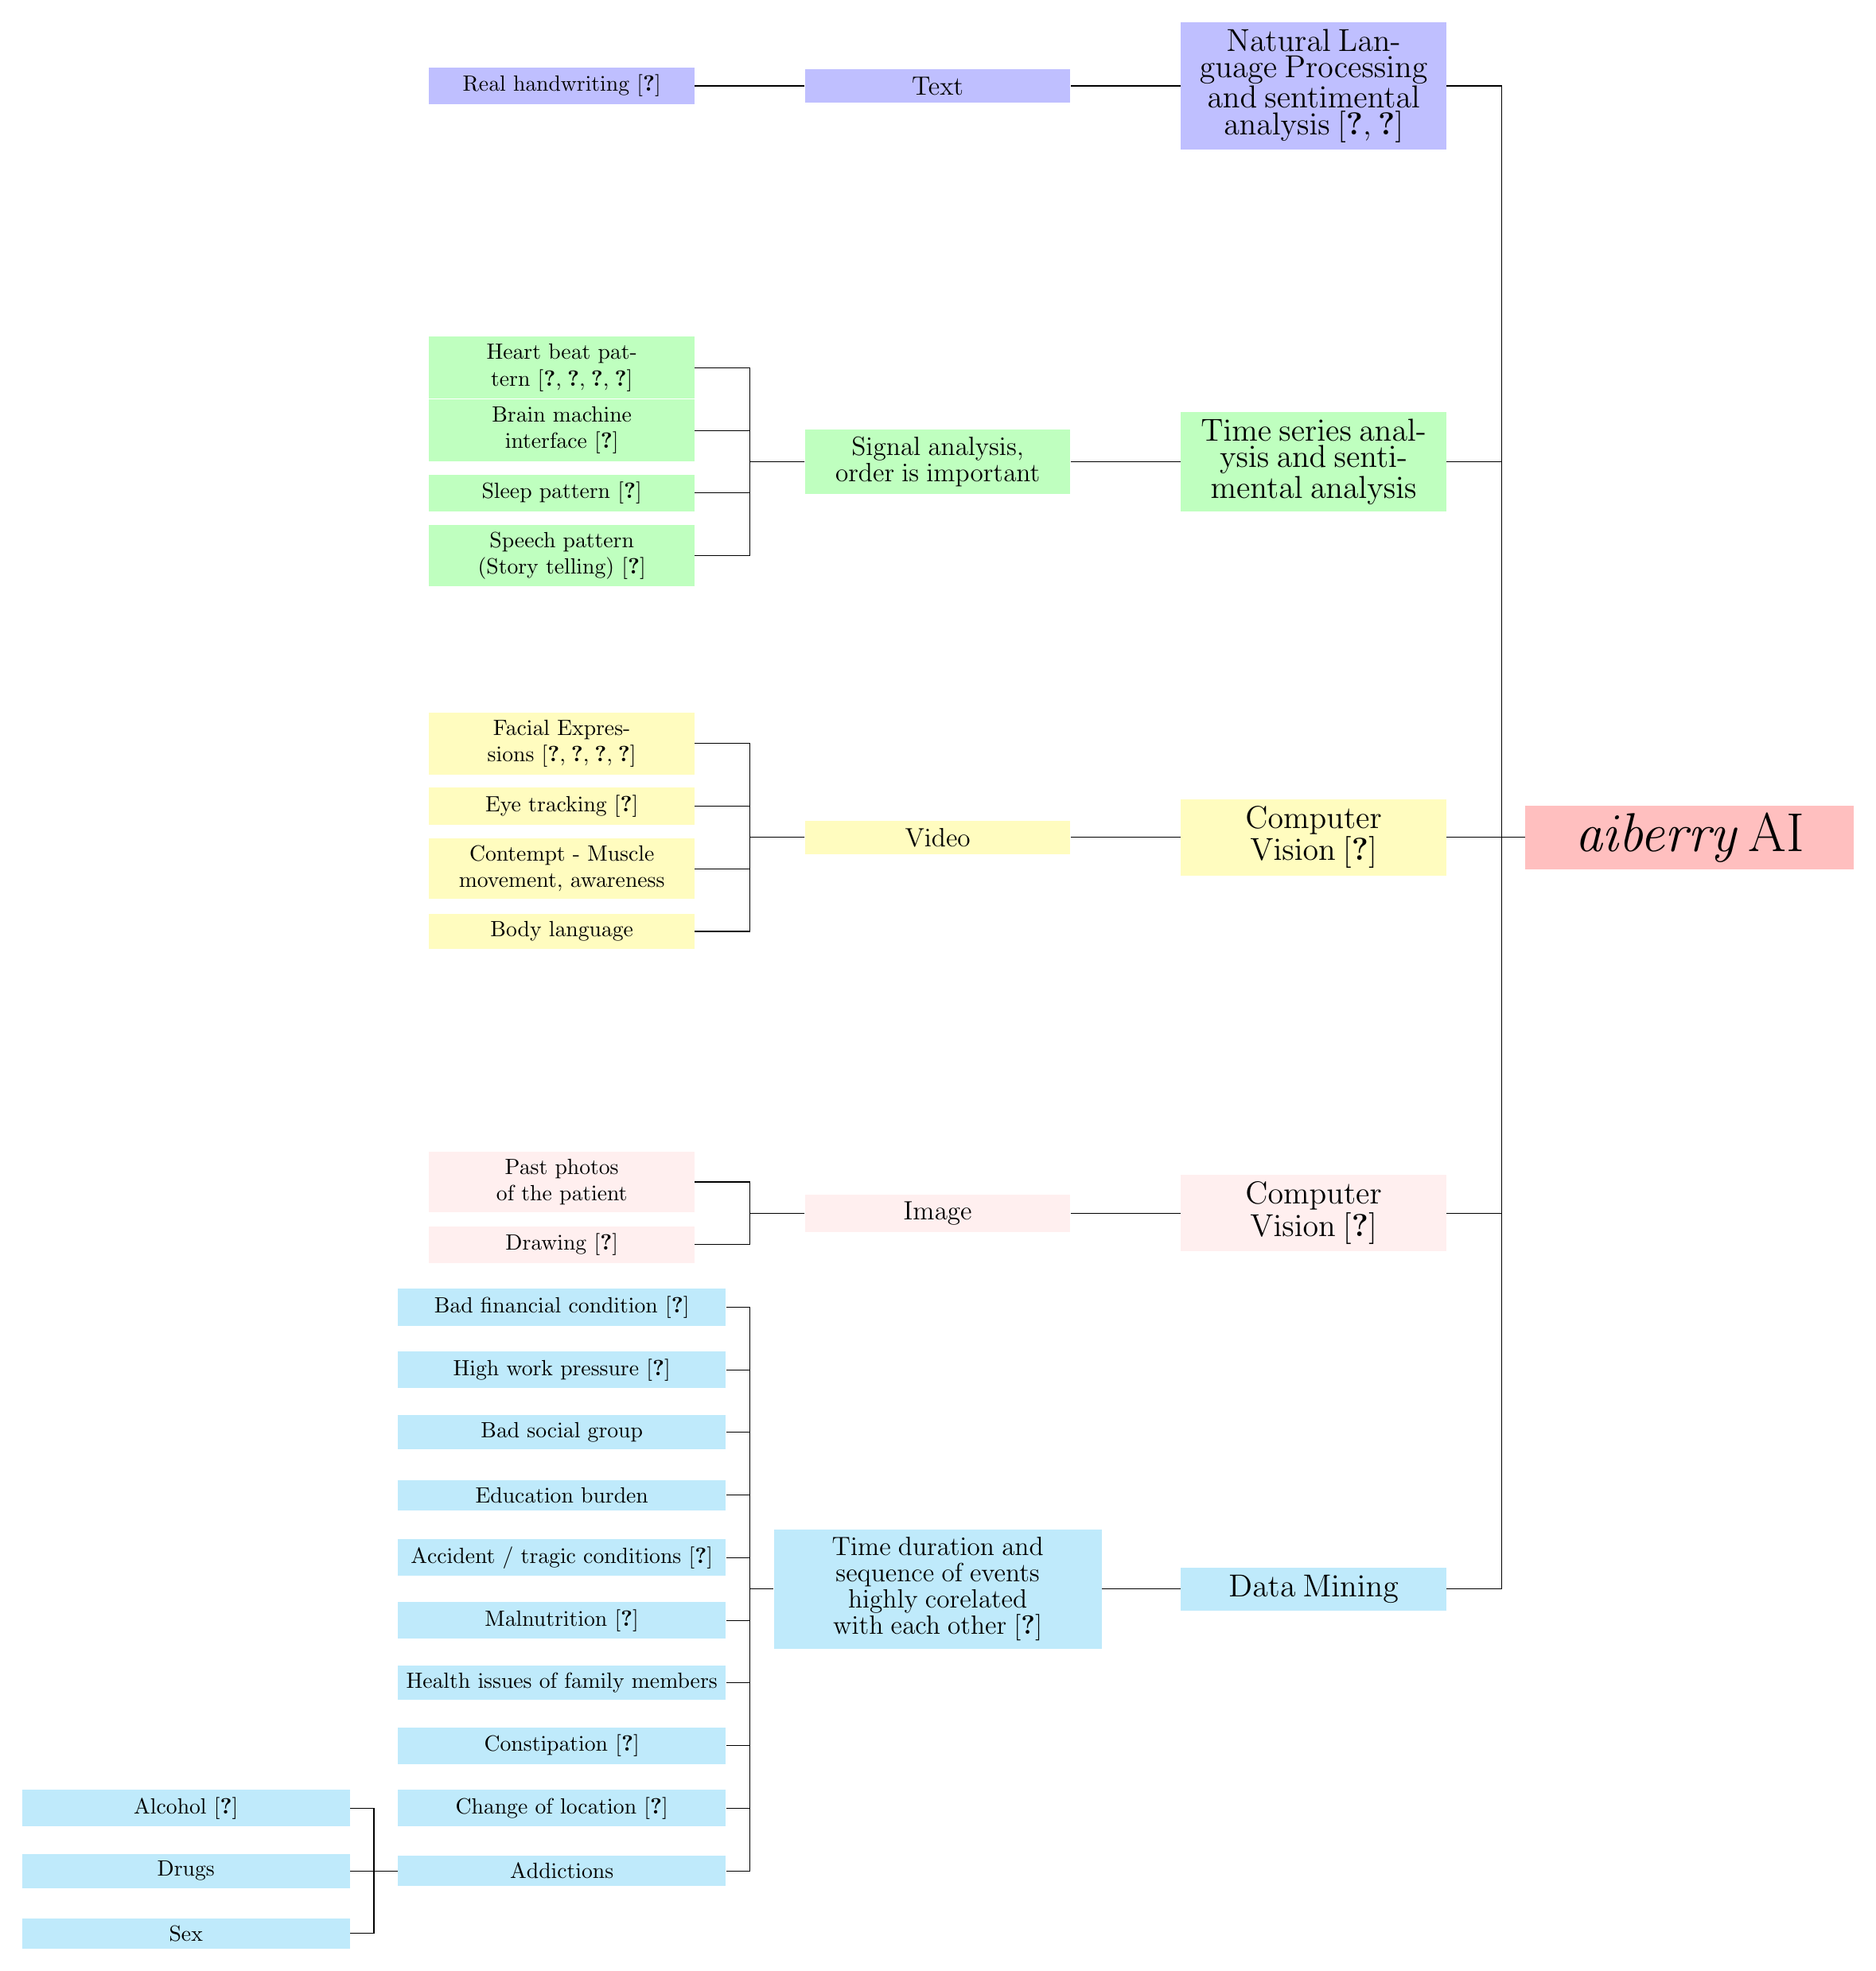
\begin{tikzpicture}[edge from parent fork left,grow=left,level distance=6cm,level 1/.style={sibling distance=6cm},
level 2/.style={sibling distance=1cm}, level 3/.style={sibling distance=1cm}]
\node[align=center, fill=red!25, text width=5cm] {\Huge \textit{aiberry} AI}
child {node [align=center, fill=blue!25,text width=4cm]{\Large Natural Language Processing and sentimental analysis \cite{nlphoward2013approach,bourla2018ptsd}}
	child {node [align=center, fill=blue!25,text width=4cm]{\large Text}
			child {node [align=center, fill=blue!25,text width=4cm]{Real handwriting \cite{handwriting2015}}}}}
%			child {node [align=center, fill=blue!25,text width=4cm]{Digital}}}}
child {node [align=center, fill=green!25,text width=4cm]{\Large Time series analysis and sentimental analysis}
	child {node [align=center, fill=green!25,text width=4cm]{\large Signal analysis, order is important}
		child {node [align=center, fill=green!25,text width=4cm]{Heart beat pattern \cite{heart2016,heartsmokealcohol2014,heart2010riganello, heartkibler2009hypertension}}}
		child {node [align=center, fill=green!25,text width=4cm]{Brain machine interface \cite{brainsignals2019butt}}}
		child {node [align=center, fill=green!25,text width=4cm]{Sleep pattern \cite{heartsmokealcohol2014}}}
		child {node [align=center, fill=green!25,text width=4cm]{Speech pattern (Story telling) \cite{speechvan2010telling}}}}}
child {node [align=center, fill=yellow!25,text width=4cm]{\Large Computer Vision \cite{cosic2013computer}}
	child {node [align=center, fill=yellow!25,text width=4cm]{\large Video}
		child {node [align=center, fill=yellow!25,text width=4cm]{Facial Expressions \cite{facearmony2005amygdala,facegarrett2012brain,facefujiwara2015association, faceshin2006amygdala}}}
		child {node [align=center, fill=yellow!25,text width=4cm]{Eye tracking \cite{eyepowers2019attention}}}
		child {node [align=center, fill=yellow!25,text width=4cm][text width=4cm]{Contempt - Muscle movement, awareness}}
		child {node [align=center, fill=yellow!25,text width=4cm]{Body language}}}}
child {node [align=center, fill=pink!25,text width=4cm]{\Large Computer Vision \cite{cosic2013computer}}
	child {node [align=center, fill=pink!25,text width=4cm]{\large Image}
		child {node [align=center, fill=pink!25,text width=4cm]{Past photos of the patient}}
		child {node [align=center, fill=pink!25,text width=4cm]{Drawing \cite{drawingspring2004thirty}}}}}
child {node [align=center, fill=cyan!25,text width=4cm]{\Large Data Mining}
	child {node [align=center, fill=cyan!25,text width=5cm]{\large Time duration and sequence of events highly corelated with each other \cite{kessler1995posttraumatic}}
		child {node [align=center, fill=cyan!25,text width=5cm]{Bad financial condition \cite{financialptsd2005}}}
		child {node [align=center, fill=cyan!25,text width=5cm]{High work pressure \cite{workchan2004influence}}}
		child {node [align=center, fill=cyan!25,text width=5cm]{Bad social group}}
		child {node [align=center, fill=cyan!25,text width=5cm]{Education burden}}
		child {node [align=center, fill=cyan!25,text width=5cm]{Accident / tragic conditions \cite{joyce2007language}}}
		child {node [align=center, fill=cyan!25,text width=5cm]{Malnutrition \cite{malnutritionde2012impact}}}
		child {node [align=center, fill=cyan!25,text width=5cm]{Health issues of family members}}
		child {node [align=center, fill=cyan!25,text width=5cm]{Constipation \cite{ibsptsd2019}}}
		child {node [align=center, fill=cyan!25,text width=5cm]{Change of location \cite{joyce2007language}}}
		child {node [align=center, fill=cyan!25,text width=5cm]{Addictions}
			child {node [align=center, fill=cyan!25,text width=5cm]{Alcohol \cite{heartsmokealcohol2014}}}
			child {node [align=center, fill=cyan!25,text width=5cm]{Drugs}}
			child {node [align=center, fill=cyan!25,text width=5cm]{Sex}}}}};
\end{tikzpicture}
\end{subgroup}
\end{table}
%\bibliographystyle{srt}
%\input{mindmaps2.bbl}
%
\bibliographystyle{ieeetr}
\Large
%\bibliographystyle{ieeetran}
\bibliography{ref}
\end{document}
%
\bibliographystyle{ieeetr}
\Large
%\bibliographystyle{ieeetran}
\bibliography{ref}
\end{document}
%
\bibliographystyle{ieeetr}
\Large
%\bibliographystyle{ieeetran}
\bibliography{ref}
\end{document}
%
\bibliographystyle{ieeetr}
\Large
%\bibliographystyle{ieeetran}
\bibliography{ref}
\end{document}